\chapter{Introduction}
	%  - Introduction 
			%- 	CMB 
			%- 	Cosmological Parameters
\section{Modern Cosmology, and the Cosmic Microwave Background}
Modern cosmology has been experiencing a golden age since the 1990s. Access to larger and larger datasets have allowed astronomers to develop some of the most accurate and detailed models we have. These models rely on several fundamental assumptions, stemming from observation, the chief of which is the Big Bang Model. 
\par Edwin Hubble discovered a relation between distances to galaxies and their recessional velocities, where galaxies that are further away appear to be moving away from us faster than those that are closer to us. His observations gave rise to the Hubble Law,
\begin{equation}
	v  \varpropto d
	\label{eq:HubbleLaw}
\end{equation}
where $v$ is the velocity of the galaxy in question, and $d$ is its distance from us. Now, there is nothing that suggests that our position in the universe is special or unique, a concept known as the Copernican Principle. This leads to the logical extension that if every point in the universe is moving away from every other point,  the universe must have been an incredibly hot, dense environment at some point in the past. Using general relativity, the extrapolation backwards in time yields a singularity of infinite density and temperature, which is commonly called the \emph{Big Bang}.
\par This singularity then expanded, exponentially growing and cooling the burgeoning universe. Small scale fluctuations in 
\par Another assumption stemming from observation is that of isotropy. Based on observation, there appears to be no favoured direction in the universe, since distributions of distant galaxies and other extragalactic sources seem to be evenly distributed across the sky. Perhaps the most spectacular example of this isotropy is the presence of the \emph{Cosmic Microwave Background}.
\par Discovered in 1964 \citep{Penzias:65}, it was noticed that there was isotropic black-body radiation at $T \approx \SI{2.7}{\kelvin}$. Since the peak of this radiation is in the microwave section of the electromagnetic spectrum, it was termed the \emph{Cosmic Microwave Background}.
\begin{figure}[ht]
	\centering
	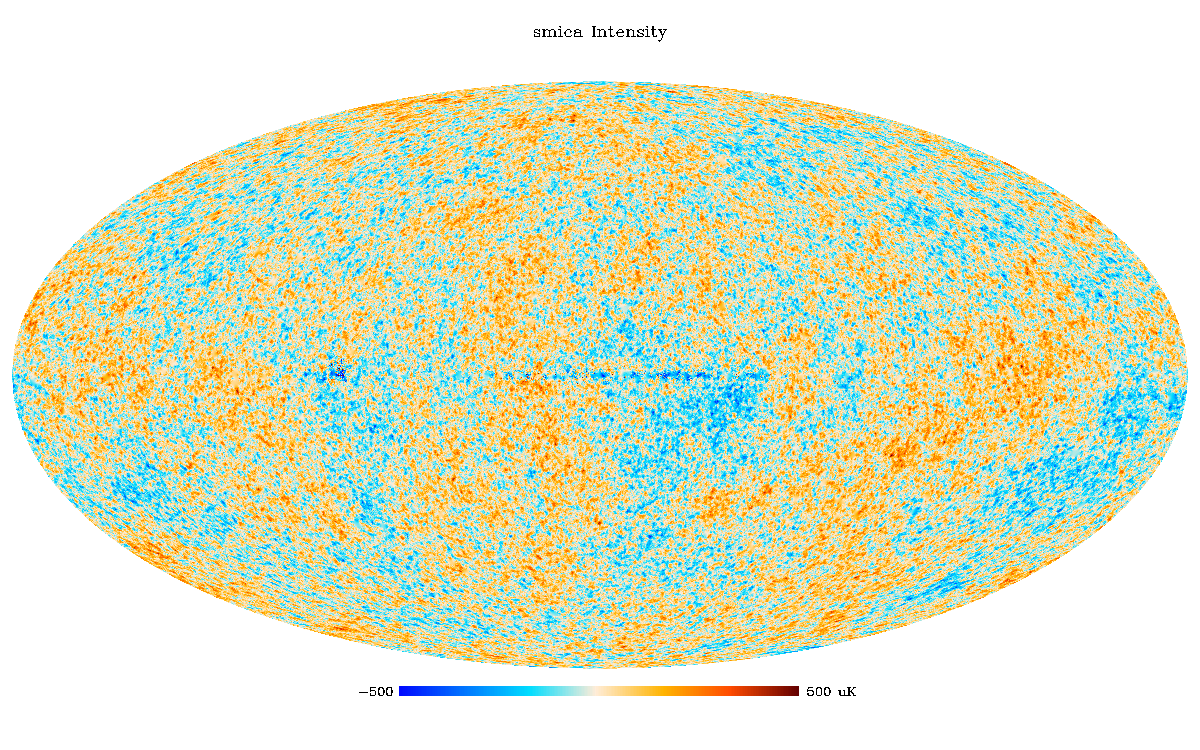
\includegraphics[scale=0.25]{/home/mitchell/Documents/masters/masters/thesis/Images/CMB_smica_tsig.png}
	\label{CMB Map}
	\caption{\emph{Planck} Satellite Full Sky CMB Map, extracted using the SMICA method. This  method linearly combines the full spectrum of frequencies observed by the \emph{Planck} satellite from $\SI{30}{\giga\hertz}$ to $\SI{857}{\giga\hertz}$ in frequency space. Each map is first converted to its power spectrum, and then weighted at various multipoles, in order to account for contamination which appears at characteristic scales in different frequencies.}
\end{figure}

The Cosmic Microwave Background (CMB) is a near-perfectly uniform field of background radiation, which as its name suggests, sits primarily within the microwave part of the electromagnetic spectrum. It is the closest measurement we have to a perfect black-body, with variations to approximately one part in $100000$, with an RMS of $\SI{18}{\micro\kelvin}$ \cite{2004mmu..symp..291W}. 

Theory holds that a very short time after the Big Bang ($\sim 10^{-37}$ seconds), the universe underwent an exponential growth period now termed \textit{inflation}. This phase is necessary to ensure that the universe is isotropic, whilst also still taking into account the apparent causal disconnect between different edges of the universe. During this period, the universe was smoothed out, only leaving behind irregularities that originated with quantum fluctuations in the scalar field that drove it. These irregularities are what eventually gives rise to the large scale structure of the universe. 

As the universe adiabatically cooled, there was a considerable period of time, until approximately $380000$ years after the Big Bang, where photons were coupled to the other components of the universe, such as the baryonic and dark matter. This period is what allowed for the quark-gluon plasma to mix appropriately, and develop sound waves, ultimately resulting in the characterstic pattern in the CMB. This pattern is highly dependant on statistical parameters, and so the characterisitic angular size of the pattern of the CMB is incredibly sensitive to the relative proportions of the universe's matter-energy density. These charactersitic angular splotches can be decomposed into a power spectrum, which exibits a shape highly dependant on universal parameters.

\begin{figure}[h!]
\centering
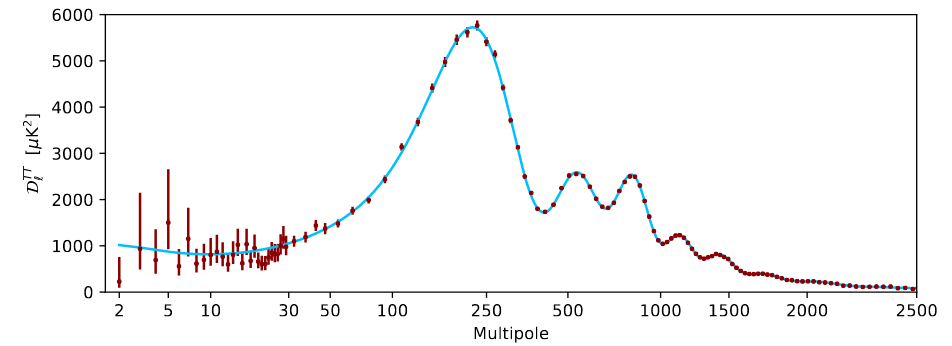
\includegraphics[scale=0.4]{/home/mitchell/Documents/masters/masters/thesis/Ver_2/figures/planck_2018.png}
\caption{\emph{Planck} 2018 Angular Power Spectrum \citep{2018arXiv180706209P}. The location, and relative heights of the first three peaks are sensitive to the overall energy density of the universe, as well as the relative amounts of baryonic matter and dark matter.}
\end{figure}

The Cosmic Microwave Background (CMB) provides the most accurate and detailed measures of the primary cosmological parameters to date. 

\section{Cosmological Parameters}
For a $\Lambda+$CDM universe, there are six independant paramters which descirbe the evolution and behaviour of the universe, the physical baryon density $\Omega_b h^2$, the physical dark matter density $\Omega_c h^2$, the age of the universe $t_0$ (or its reciprocal, the Hubble constant $H_0$), the scalar spectral index $n_s$, the curvature fluctuation amplitude $\Delta_R^2$, and the reionisation optical depth $\tau$. There is also another parameter which is used frequently, known as the reduced Hubble Constant $h$, and is derived from the primary Hubble Constant. Ordinarily, if it lacks a subscript, it refers to the definition $h = H_0/\SI{100}{\kilo\meter\per\second\per\mega\parsec}$, but if it carries one, it refers to replacing the number in the denominator with the number in the subscript, e.g. $h_{70} = H_0/\SI{70}{\kilo\meter\per\second\per\mega\parsec}$.

Currently, the highest precision measures of these features from the CMB come from \cite{2018arXiv180706209P}, which details that baryonic matter only comprises $\approx 5 \% $ of the universe's energy density. In principle, this component of the universe should be directly measurable. At just three minutes after the Big Bang, deuterium can be used as a tracer for this abundance \citep{2007ARNPS..57..463S}, and at redshift $z \geqslant 2$, the baryon fraction can be found in the absorption lines of quasars passing through the diffuse, photo-ionised intergalactic medium, known as the Lyman-$\alpha$ forest \citep{1997ApJ...490..564W}. However as the universe evolved, this gas became sparser as it became more ionised. This makes searching for the entirety of the baryon fraction at low redshift difficult. When this fraction is calculated directly from observations, it shows only one tenth of the baryonic content shown in high redshift measurements is contained in galactic structures \citep{1992MNRAS.258P..14P}. Some revised estimates considered that the limitations of observations were primarily to blame for this discrepency, and not inherent new physics \citep{1994MNRAS.267...13B, 1998ApJ...503..518F}

The baryon content has been confirmed to a very high accuracy with recent CMB experiments, first with the \textit{Wilkinson Microwave Anisotropy Probe} (WMAP) \citep{2007ApJS..170..377S}, and then with the \textit{Planck} Satellite . When we quote quantities, we take values from the latest \textit{Planck} paper \cite{2018arXiv180706209P}


\begin{center}\label{table:params}
 \begin{tabular}{||c c c||} 
 \hline
 Parameter & Value & Error \\
 \hline\hline
 $\Omega_c h^2$ & $0.120$ & $\pm 0.001$ \\
 \hline
 $\Omega_b h^2$ & $0.0224$ & $\pm 0.0001$ \\
 \hline
  $n_s$ & $0.965$ & $\pm 0.004$ \\
 \hline
  $\tau$  & $0.054$ & $\pm 0.007$ \\
 \hline
  $100 \Theta_\star$ & $1.0411$ & $\pm 0.0003$ \\
 \hline
 $H_0$ (km s$^{-1}$ Mpc$^{-1}$) & $67.4$ & $\pm 0.5$ \\
 \hline
\end{tabular}
\end{center}



